\documentclass[dvips, lscape]{foils}
%\documentclass[dvips, french]{slides}
\textwidth 18.5cm
\textheight 25cm 
\topmargin -1cm 
\oddsidemargin  -1cm 
\evensidemargin  -1cm

% Maths
\usepackage{amsfonts, amsmath, amssymb}

\newcommand{\coefbin}[2]{\left( 
    \begin{array}{c} #1 \\ #2 \end{array} 
  \right)}
\newcommand{\Bcal}{\mathcal{B}}
\newcommand{\Ccal}{\mathcal{C}}
\newcommand{\Dcal}{\mathcal{D}}
\newcommand{\Ecal}{\mathcal{E}}
\newcommand{\Gcal}{\mathcal{G}}
\newcommand{\Mcal}{\mathcal{M}}
\newcommand{\Ncal}{\mathcal{N}}
\newcommand{\Pcal}{\mathcal{P}}
\newcommand{\Qcal}{\mathcal{Q}}
\newcommand{\Lcal}{\mathcal{L}}
\newcommand{\Tcal}{\mathcal{T}}
\newcommand{\Ucal}{\mathcal{U}}
\newcommand{\alphabf}{\mbox{\mathversion{bold}{$\alpha$}}}
\newcommand{\betabf}{\mbox{\mathversion{bold}{$\beta$}}}
\newcommand{\gammabf}{\mbox{\mathversion{bold}{$\gamma$}}}
\newcommand{\mubf}{\mbox{\mathversion{bold}{$\mu$}}}
\newcommand{\thetabf}{\mbox{\mathversion{bold}{$\theta$}}}
\newcommand{\Pibf}{\mbox{\mathversion{bold}{$\Pi$}}}
\newcommand{\psibf}{\mbox{\mathversion{bold}{$\psi$}}}
\newcommand{\Sigmabf}{\mbox{\mathversion{bold}{$\Sigma$}}}
\newcommand{\taubf}{\mbox{\mathversion{bold}{$\tau$}}}
\newcommand{\Ebf}{{\bf E}}
\newcommand{\Gbf}{{\bf G}}
\newcommand{\Hbf}{{\bf H}}
\newcommand{\Ibf}{{\bf I}}
\newcommand{\mbf}{{\bf m}}
\newcommand{\Obf}{{\bf 0}}
\newcommand{\Rbf}{{\bf R}}
\newcommand{\Sbf}{{\bf S}}
\newcommand{\Tbf}{{\bf T}}
\newcommand{\Ubf}{{\bf U}}
\newcommand{\Vbf}{{\bf V}}
\newcommand{\xbf}{{\bf x}}
\newcommand{\Xbf}{{\bf X}}
\newcommand{\Ybf}{{\bf Y}}
\newcommand{\Zbf}{{\bf Z}}
\newcommand{\Esp}{{\mathbb E}}
\newcommand{\Var}{{\mathbb V}}
\newcommand{\Cov}{{\mathbb C}\mbox{ov}}
\newcommand{\Ibb}{{\mathbb I}}
\newcommand{\Rbb}{\mathbb{R}}

% sommes
\newcommand{\sumk}{\sum_k}
\newcommand{\sumt}{\sum_{t \in I_k}}
\newcommand{\sumth}{\sum_{t=t_{k-1}^{(h)}+1}^{t_k^{(h)}}}
\newcommand{\sump}{\sum_{p=1}^{P}}
\newcommand{\suml}{\sum_{\ell=1}^{P}}
\newcommand{\sumtau}{\sum_k \hat{\tau}_{kp}}

% Couleur et graphiques
\usepackage{color}
\usepackage{graphics}
\usepackage{epsfig} 
\usepackage{pstcol}

% Texte
\usepackage{lscape}
\usepackage{../../../../Latex/fancyheadings, rotating, enumerate}
%\usepackage[french]{babel}
\usepackage[latin1]{inputenc}
\definecolor{darkgreen}{cmyk}{0.5, 0, 0.5, 0.5}
\definecolor{orange}{cmyk}{0, 0.6, 0.8, 0}
\definecolor{jaune}{cmyk}{0, 0.5, 0.5, 0}
\newcommand{\textblue}[1]{\textcolor{blue}{#1}}
\newcommand{\textred}[1]{\textcolor{red}{#1}}
\newcommand{\textgreen}[1]{\textcolor{green}{ #1}}
\newcommand{\textlightgreen}[1]{\textcolor{green}{#1}}
%\newcommand{\textgreen}[1]{\textcolor{darkgreen}{#1}}
\newcommand{\textorange}[1]{\textcolor{orange}{#1}}
\newcommand{\textyellow}[1]{\textcolor{yellow}{#1}}
\newcommand{\refer}[2]{{\sl #1}}
\newcommand{\emphase}[1]{\textblue{\sl #1}}

% Sections
%\newcommand{\chapter}[1]{\centerline{\LARGE \textblue{#1}}}
% \newcommand{\section}[1]{\centerine{\Large \textblue{#1}}}
% \newcommand{\subsection}[1]{\noindent{\Large \textblue{#1}}}
% \newcommand{\subsubsection}[1]{\noindent{\large \textblue{#1}}}
% \newcommand{\paragraph}[1]{\noindent {\textblue{#1}}}
% Sectionsred
\newcommand{\chapter}[1]{
  \addtocounter{chapter}{1}
  \setcounter{section}{0}
  \setcounter{subsection}{0}
  {\centerline{\LARGE \textblue{\arabic{chapter} - #1}}}
  }
\newcommand{\section}[1]{
  \addtocounter{section}{1}
  \setcounter{subsection}{0}
  {\centerline{\Large \textblue{\arabic{chapter}.\arabic{section} - #1}}}
  }
\newcommand{\subsection}[1]{
  \addtocounter{subsection}{1}
  {\noindent{\large \textblue{#1}}}
  }
% \newcommand{\subsection}[1]{
%   \addtocounter{subsection}{1}
%   {\noindent{\large \textblue{\arabic{chapter}.\arabic{section}.\arabic{subsection} - #1}}}
%   }
\newcommand{\paragraph}[1]{\noindent{\textblue{#1}}}

%%%%%%%%%%%%%%%%%%%%%%%%%%%%%%%%%%%%%%%%%%%%%%%%%%%%%%%%%%%%%%%%%%%%%%
%%%%%%%%%%%%%%%%%%%%%%%%%%%%%%%%%%%%%%%%%%%%%%%%%%%%%%%%%%%%%%%%%%%%%%
%%%%%%%%%%%%%%%%%%%%%%%%%%%%%%%%%%%%%%%%%%%%%%%%%%%%%%%%%%%%%%%%%%%%%%
%%%%%%%%%%%%%%%%%%%%%%%%%%%%%%%%%%%%%%%%%%%%%%%%%%%%%%%%%%%%%%%%%%%%%%
\begin{document}
%%%%%%%%%%%%%%%%%%%%%%%%%%%%%%%%%%%%%%%%%%%%%%%%%%%%%%%%%%%%%%%%%%%%%%
%%%%%%%%%%%%%%%%%%%%%%%%%%%%%%%%%%%%%%%%%%%%%%%%%%%%%%%%%%%%%%%%%%%%%%
%%%%%%%%%%%%%%%%%%%%%%%%%%%%%%%%%%%%%%%%%%%%%%%%%%%%%%%%%%%%%%%%%%%%%%
%%%%%%%%%%%%%%%%%%%%%%%%%%%%%%%%%%%%%%%%%%%%%%%%%%%%%%%%%%%%%%%%%%%%%%
\landscape
\newcounter{chapter}
\newcounter{section}
\newcounter{subsection}
\setcounter{chapter}{0}
\headrulewidth 0pt 
\pagestyle{fancy} 
\cfoot{}
\rfoot{\begin{rotate}{90}{
      \hspace{1cm} \tiny S. Robin: Segmentation-clustering for CGH
      }\end{rotate}}
\rhead{\begin{rotate}{90}{
      \hspace{-.5cm} \tiny \thepage
      }\end{rotate}}

%%%%%%%%%%%%%%%%%%%%%%%%%%%%%%%%%%%%%%%%%%%%%%%%%%%%%%%%%%%%%%%%%%%%%%
%%%%%%%%%%%%%%%%%%%%%%%%%%%%%%%%%%%%%%%%%%%%%%%%%%%%%%%%%%%%%%%%%%%%%%
\begin{center}
  \textblue{\LARGE Statistical Analysis of CGH Arrays}

   \vspace{1cm}
   {\large F. Picard, S. Robin, E. Lebarbier, J-J. Daudin} \\
   robin@inapg.inra.fr

   {UMR INA-PG / ENGREF / INRA, Paris} \\
   {Math�matique et Informatique Appliqu�es}
   
    \vspace{1cm}
    {Monolix, October 2006}
\end{center}

%\vspace{2cm}
\paragraph{Outline}

1 - Microarray CGH technology 

2 - Breakpoint detection  

3 - Multiple arrays analysis

%%%%%%%%%%%%%%%%%%%%%%%%%%%%%%%%%%%%%%%%%%%%%%%%%%%%%%%%%%
%%%%%%%%%%%%%%%%%%%%%%%%%%%%%%%%%%%%%%%%%%%%%%%%%%%%%%%%%%%%%
\newpage
\chapter{Detection of chromosomal aberrations}
%%%%%%%%%%%%%%%%%%%%%%%%%%%%%%%%%%%%%%%%%%%%%%%%%%%%%%%%%%%%%
%%%%%%%%%%%%%%%%%%%%%%%%%%%%%%%%%%%%%%%%%%%%%%%%%%%%%%%%%%

%%%%%%%%%%%%%%%%%%%%%%%%%%%%%%%%%%%%%%%%%%%%%%%%%%%%%%%%%%
\vspace{1cm}
\section{Aberration at the chromosomic scale}
%%%%%%%%%%%%%%%%%%%%%%%%%%%%%%%%%%%%%%%%%%%%%%%%%%%%%%%%%%

Known effects of big size chromosomal aberrations  (ex:
trisomy).

\centerline{$\rightarrow$ experimental tool: \textblue{Karyotype}
  (Resolution $\sim$ chromosome)} 

$$
\epsfig{file = ../Figures/Karyotype.ps, clip=,
  bbllx=158, bblly=560, bburx=452, bbury=778, scale=1.2}
$$

%%%%%%%%%%%%%%%%%%%%%%%%%%%%%%%%%%%%%%%%%%%%%%%%%%%%%%%%%%
\newpage
\section{Within chromosome aberration}
%%%%%%%%%%%%%%%%%%%%%%%%%%%%%%%%%%%%%%%%%%%%%%%%%%%%%%%%%%
\begin{itemize}
\item Change of scale: what are the effects of small size DNA
  sequences deletions/amplifications?\\
%  \\
  \centerline{$\rightarrow$ experimental tool:
    \textblue{"conventional" CGH} (resolution $\sim$ 10Mb).}
\item CGH = Comparative Genomic Hybridization: method for the
  comparative measurement of relative DNA copy numbers between two
  samples (normal/disease, test/reference).\\ 
%  \\
  \centerline{$\rightarrow$ Application of the \textblue{microarray}
    technology to CGH (resolution $\sim$ 100kb).}
  $$
  \epsfig{file = ../Figures/CGHarray.ps, clip=,
    bbllx=113, bblly=564, bburx=497, bbury=778, scale=1.1}
  $$
\end{itemize}

%%%%%%%%%%%%%%%%%%%%%%%%%%%%%%%%%%%%%%%%%%%%%%%%%%%%%%%%%%%%%
\newpage
\section{Microarray technology in its principle }
%%%%%%%%%%%%%%%%%%%%%%%%%%%%%%%%%%%%%%%%%%%%%%%%%%%%%%%%%%%%%
\vspace{-1cm}
$$
\epsfig{file = ../Figures/principe_CGH.eps, clip=,
  bbllx=0, bblly=41, bburx=700, bbury=478, scale=0.9}
$$

%%%%%%%%%%%%%%%%%%%%%%%%%%%%%%%%%%%%%%%%%%%%%%%%%%%%%%%%%%%%%
\newpage
\section{Interpretation of a CGH profile }
%%%%%%%%%%%%%%%%%%%%%%%%%%%%%%%%%%%%%%%%%%%%%%%%%%%%%%%%%%%%%
\vspace{-0.5cm}
$$
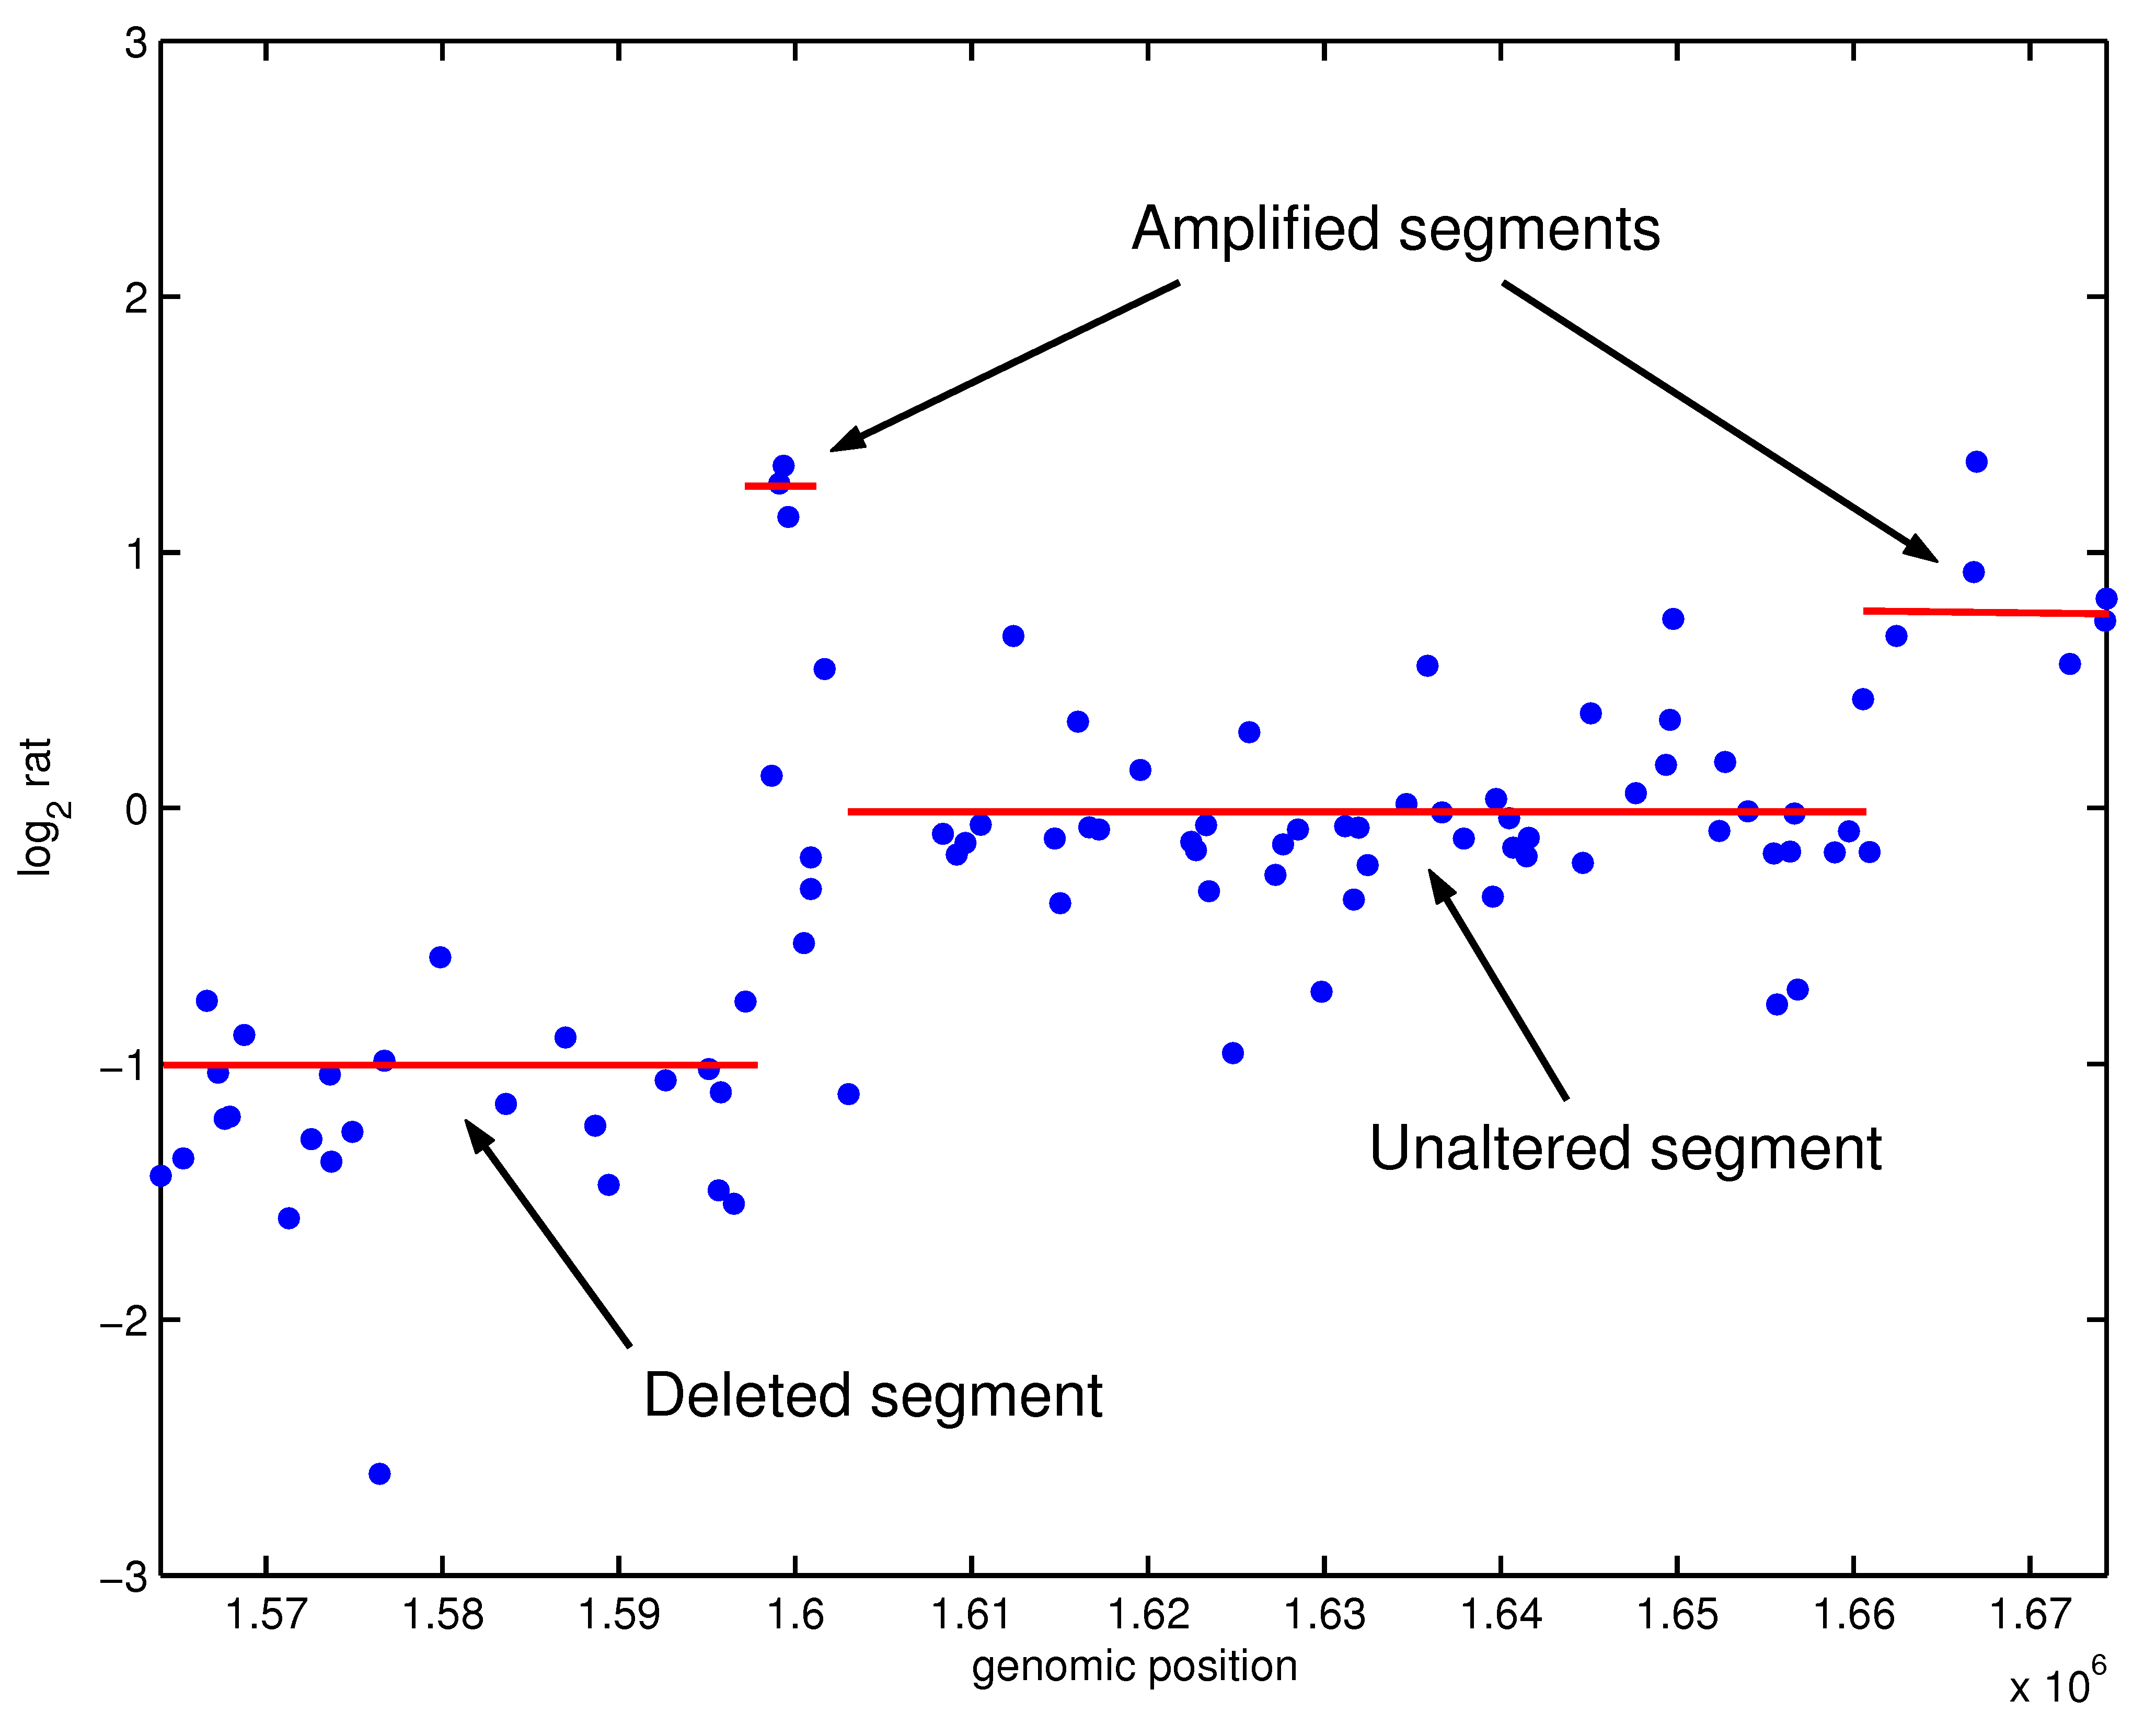
\epsfig{file = ../Figures/profile_example.eps, clip=,
  bbllx=60, bblly=196, bburx=543, bbury=586}
$$
\centerline{
  A dot on the graph 
  $
  \displaystyle{
    = \log_2 \left\{ \frac{\text{ $\sharp$ copies of BAC(t) in the test
          genome }}{\text{$\sharp$ copies of BAC(t) in the reference
          genome}}\right\}}
  $
}

%%%%%%%%%%%%%%%%%%%%%%%%%%%%%%%%%%%%%%%%%%%%%%%%%%%%%%%%%%
%%%%%%%%%%%%%%%%%%%%%%%%%%%%%%%%%%%%%%%%%%%%%%%%%%%%%%%%%%
\newpage
\chapter{Breakpoint detection}
%%%%%%%%%%%%%%%%%%%%%%%%%%%%%%%%%%%%%%%%%%%%%%%%%%%%%%%%%%
%%%%%%%%%%%%%%%%%%%%%%%%%%%%%%%%%%%%%%%%%%%%%%%%%%%%%%%%%%
%%%%%%%%%%%%%%%%%%%%%%%%%%%%%%%%%%%%%%%%%%%%%%%%%%%%%%%%%
\bigskip
\section{What do we have in mind?}
%%%%%%%%%%%%%%%%%%%%%%%%%%%%%%%%%%%%%%%%%%%%%%%%%%%%%%%%%%

\begin{itemize}
\item At position $t$, there exists a 'true' log-ratio $\lambda_t$,
  which depends on the relative copy number.
\item The value of the true log-ratio $\lambda_t$ is affected by
  abrupt changes:
                                %\vspace{-0.5cm}
  $$
  \epsfig{file = ../Figures/FigSeg_Intro.eps, clip=, bbllx=90,
    bblly=300, bburx=540, bbury=400, scale = 1.2}
  $$
  Position \paragraph{$t_1$, $t_2$, ..} are called {\sl
    breakpoints}. \paragraph{$\mu_k$} is the true log-ratio in segment
  \paragraph{$I_k$}.
\item The observed signal $Y_t$ is noisy:
  $$
  Y_t = \lambda_t + E_t.
  $$
%   where $\lambda_t$ is the true log-ratio and $E_t$ is a noise
%   (typically, $E_t \sim \Ncal(0, \sigma^2)$).
\end{itemize}

%%%%%%%%%%%%%%%%%%%%%%%%%%%%%%%%%%%%%%%%%%%%%%%%%%%%%%%%%%
\newpage
%\bigskip
\section{Statistical model} 
%%%%%%%%%%%%%%%%%%%%%%%%%%%%%%%%%%%%%%%%%%%%%%%%%%%%%%%%%%
\vspace{-0.5cm}\begin{itemize}
\item The breakpoints define a partition of the data into $K$
  segments of size $n_k$:
  $$
  I_k=\{t, t \in ]t_{k-1},t_k]\}, 
  \qquad
  Y^k=\{Y_t, t \in I_k\}.
  $$
\item Suppose that those parameters are constant between two changes:
  $$
  \mbox{if position $t$ is in segment $I_k$,} \qquad Y_t = \mu_k +
  E_t \sim \Ncal(\mu_k,\sigma_{(k)}^2).
  $$
\item The parameters of this model are: 
  $$
  T  =  (t_1, ..., t_{K-1}),
  \qquad
  \Theta  = (\theta_1,\hdots,\theta_K), \quad \theta_k=(\mu_k,\sigma_{(k)}^2).
  $$
\end{itemize}
Breakpoints detection aims at studying the \textblue{spatial structure
  of the signal}.

%%%%%%%%%%%%%%%%%%%%%%%%%%%%%%%%%%%%%%%%%%%%%%%%%%%%%%%%%%
\newpage
\subsection{Estimating the parameters}
%%%%%%%%%%%%%%%%%%%%%%%%%%%%%%%%%%%%%%%%%%%%%%%%%%%%%%%%%%

\paragraph{Log-Likelihood} (with a constant variance $\sigma^2$):
\begin{eqnarray*}
2 \Lcal_K(T, \Theta) & = & 2 \sum_{k=1}^K \log \phi(\{Y_t\}_{t \in I_k};
\theta_k) \quad = \quad 2 \sum_{k=1}^K \sum_{t \in I_k}\log \phi(Y_t; \theta_k) \\
& = & -n \log \sigma^2 - \frac1{\sigma^2} \sum_{k=1}^K \sum_{t \in
  I_k} (Y_t - \mu_k)^2 + \mbox{cst}. 
\end{eqnarray*}

\paragraph{2 important remarks:}
\begin{enumerate}
\item Because the data are supposed to be independent, the
log-likelihood is a sum over all the segments (\emphase{additive
contrast}).
\item Because the data are supposed to be Gaussian, maximum likelihood
  estimation is equivalent to least square fitting.
\end{enumerate}

%%%%%%%%%%%%%%%%%%%%%%%%%%%%%%%%%%%%%%%%%%%%%%%%%%%%%%%%%%
\newpage
\paragraph{When the breakpoints are known.}
Since we are in a Gaussian framework, maximum likelihood is equivalent
to least square estimate, so we get for the mean:
$$
\widehat{\mu}_k = \frac1{n_k} \sum_{t \in I_k} Y_t
$$
and for the variance,
\begin{itemize}
\item if it is supposed to be constant along the whole chromosome:
  $$
  \widehat{\sigma}^2 =  \frac1{n} \sum_{k=1}^K \sum_{t \in I_k} (Y_t -
  \widehat{\mu}_k)^2 
  $$
\item if it is supposed to be specific to each segment:
  $$
  \widehat{\sigma}^2_k = \frac1{n_k} \sum_{t \in I_k} (Y_t -
  \widehat{\mu}_k)^2 
  $$
\end{itemize}

%%%%%%%%%%%%%%%%%%%%%%%%%%%%%%%%%%%%%%%%%%%%%%%%%%%%%%%%%%
\newpage
\subsection{How to find the breakpoints?}

When $K$ is known , we have to minimise
$$
J_k(1, n) = \sum_{k=1}^K \sum_{t \in I_k} (Y_t - \widehat{\mu}_k)^2.
$$
\begin{itemize}
\item There are $\coefbin{n-1}{K-1}$ possible choices for the
  positions of the breakpoints $t_1, t_2, \dots, t_{K-1}$: \\
  \\
  \centerline{$\Rightarrow$ Impossible to explore for large
    $n$ and $K$}
\item $\sum_{t \in I_k} (Y_t - \widehat{\mu}_k)^2$ can be viewed as
  the 'cost' of segment $I_k$, i.e. the cost of putting data
  $Y_{t_{k-1}+1}$ to $Y_{t_{k+1}}$ in a single segment.
\item The optimisation problem is actually a shortest path problem
  that can be solved thanks to \paragraph{dynamic programming}.
\end{itemize}

%%%%%%%%%%%%%%%%%%%%%%%%%%%%%%%%%%%%%%%%%%%%%%%%%%%%%%%%%%
\newpage
\paragraph{Dynamic programming.} Based on Bellmann's optimality
principle: \\
\\
\centerline{\sl Sub-paths of the optimal path are themselves optimal.}

\begin{description}
\item[Initialisation:] For $0 \leq i < j \leq n$:
  $$
  J_1(i, j) = \sum_{t=i+1}^j (Y_t - \widehat{\mu})^2.
  $$
\item[Step $k$:] For $2 \leq k \leq K$:
  $$
  J_k(i, j) = \min_{i \leq h \leq j} \left[J_{k-1}(1, h) + J_1(h+1,
      j)\right].
  $$
  $J_k$ is called the \textblue{cost matrix}.
\end{description}

\paragraph{Remark:} Same principle as the Smith-Watermann algorithm
for sequence alignment.

%%%%%%%%%%%%%%%%%%%%%%%%%%%%%%%%%%%%%%%%%%%%%%%%%%%%%%%%%%
\newpage
\subsection{One last problem: the selection of $K$}

\noindent
\begin{tabular}{cc}
  \begin{tabular}{p{11cm}}
    \begin{itemize}
    \item The contrast $J_K$ necessarily decreases when the model
      becomes more complex. 
    \item The penalty function measures this complexity: $pen(K) = $
      $K+1$ with constant variance, $2K$ with heterogeneous variance.
    \item We look for the minimum of
      $$
      J_k + \beta pen(K)
      $$
      where $\beta$ is adaptively estimated ({\sl Lavielle(2003)}).
    \end{itemize}
  \end{tabular}
  &
  \begin{tabular}{c}
    \epsfig{file = ../Figures/Select_K.ps, clip=, bbllx=146, bblly=529,
      bburx=464, bbury=777, width=12cm, height=12cm} 
  \end{tabular}
\end{tabular}

%%%%%%%%%%%%%%%%%%%%%%%%%%%%%%%%%%%%%%%%%%%%%%%%%%%%%%%%%%
\newpage
\section{Example of segmentation on array CGH data}
%%%%%%%%%%%%%%%%%%%%%%%%%%%%%%%%%%%%%%%%%%%%%%%%%%%%%%%%%%

\paragraph{Are the variances $\sigma^2_k$ homogeneous?} BT474 cell
line, chromosome 9: 
$$
\begin{tabular}{cc}
  Homogeneous variances & Heterogeneous variances \\
  \multicolumn{2}{c}{$K=4$ segments} \\
  \epsfig{file = ../Figures/bt474_c9_seg_homo_K4.eps, clip=, scale=0.7} &
  \epsfig{file = ../Figures/bt474_c9_seg_hetero_K4.eps, clip=, scale=0.7} \\
\end{tabular}
$$

%%%%%%%%%%%%%%%%%%%%%%%%%%%%%%%%%%%%%%%%%%%%%%%%%%%%%%%%%%
\newpage
\paragraph{Adaptive choice of the number of segments.} BT474 cell
line, chromosome 1:
$$
\begin{tabular}{cc}
  Homogeneous variances & Heterogeneous variances \\
  $\widehat{K} = 10$  segments & $\widehat{K} = 2$ segments \\
  \epsfig{file = ../Figures/bt474_c1_seg_homo_K10.eps, clip=, scale=0.7} &
  \epsfig{file = ../Figures/bt474_c1_seg_hetero_K2.eps, clip=, scale=0.7} \\
\end{tabular}
$$
Homogeneous variances result in smaller segments.

%%%%%%%%%%%%%%%%%%%%%%%%%%%%%%%%%%%%%%%%%%%%%%%%%%%%%%%%%%
\newpage
\subsection{Comparative study} 

\paragraph{Lai \& al. (Bioinformatics, 05).} On both synthetic and
real data (GBM brain tumor data), the methods performs well.
$$
%\epsfig{file = ../Figures/LPJ05-Fig1.eps, clip=, scale=1.2}
%\epsfig{file = ../Figures/LPJ05-Fig3.eps, clip=, scale=1.2}
\epsfig{file = ../Figures/LPJ05-Fig4.eps, clip=, scale=1.2}
$$


%%%%%%%%%%%%%%%%%%%%%%%%%%%%%%%%%%%%%%%%%%%%%%%%%%%%%%%%%%
\newpage
\paragraph{ROC curves.} The sensitivity decreases for small segments
when  signal-to-noise ratio (SNR) is small.
$$
\epsfig{file = ../Figures/LPJ05-Fig2.eps, clip=, scale=1.2}
$$

%%%%%%%%%%%%%%%%%%%%%%%%%%%%%%%%%%%%%%%%%%%%%%%%%%%%%%%%%%
%%%%%%%%%%%%%%%%%%%%%%%%%%%%%%%%%%%%%%%%%%%%%%%%%%%%%%%%%%
\newpage
\chapter{Multiple arrays analysis}
\bigskip\bigskip
%%%%%%%%%%%%%%%%%%%%%%%%%%%%%%%%%%%%%%%%%%%%%%%%%%%%%%%%%%
%%%%%%%%%%%%%%%%%%%%%%%%%%%%%%%%%%%%%%%%%%%%%%%%%%%%%%%%%%

%%%%%%%%%%%%%%%%%%%%%%%%%%%%%%%%%%%%%%%%%%%%%%%%%%%%%%%%%%
\section{Problem}
%%%%%%%%%%%%%%%%%%%%%%%%%%%%%%%%%%%%%%%%%%%%%%%%%%%%%%%%%%

\subsection{Two examples.}

\paragraph{1 - Comparing {\sl A. Thaliana} mutants or ecotypes.}
Chromosomal rearrangement can be detected by comparing CGH profiles
observed on individual from of the different genotypes.

\paragraph{2 - Comparing groups of patients.}
To detect chromosomal aberration associated with a specific disease
(e.g. breast cancer), we compare the profiles of healthy and ill
patients, or the profiles of group of patients with different
prognosis. \\
Data from Institut Curie (O. Delattre, Y. de Rycke)
\bigskip

\subsection{First approach: Common breakpoints.}

If all the patients of the same group have their breakpoints at the
same positions, we have to \emphase{segment a multivariate
  signal} (as many dimensions as patients). \\
If the position are assumed to be independent, this can be done with a
\emphase{generalisation of the model} presented above and with the
\emphase{same algorithm}.


%%%%%%%%%%%%%%%%%%%%%%%%%%%%%%%%%%%%%%%%%%%%%%%%%%%%%%%%%%
\newpage
\subsection{Curie dataset: Chromosome 8.} \\
\\
\begin{tabular}{ccc}
  & Good prognosis (53 patients) & Bad prognosis (81 patients) \\
  \hspace{-1cm}
  \begin{tabular}{p{2.5cm}} Number of breakpoints \end{tabular} &
  \begin{tabular}{c}
    \epsfig{file =
      /RECHERCHE/RUPTURES/Exposes/Figures/CurieChromo8Gp1_K.eps, clip=,
      width=10cm, height=6cm}
  \end{tabular} 
  &
  \begin{tabular}{c}
    \epsfig{file =
      /RECHERCHE/RUPTURES/Exposes/Figures/CurieChromo8Gp2_K.eps, clip=,
      width=10cm, height=6cm} 
  \end{tabular} \\
  \hspace{-1cm}
  \begin{tabular}{p{2.5cm}} Position of the breakpoints \end{tabular} &
  \begin{tabular}{c}
    \epsfig{file =
      /RECHERCHE/RUPTURES/Exposes/Figures/CurieChromo8Gp1_T.eps, clip=,
      width=10cm}
  \end{tabular} 
  &
  \begin{tabular}{c}
    \epsfig{file =
      /RECHERCHE/RUPTURES/Exposes/Figures/CurieChromo8Gp2_T.eps, clip=,
      width=10cm}
  \end{tabular} 
\end{tabular}

%%%%%%%%%%%%%%%%%%%%%%%%%%%%%%%%%%%%%%%%%%%%%%%%%%%%%%%%%%
\newpage
\section{Mixed linear model with breakpoints}
%%%%%%%%%%%%%%%%%%%%%%%%%%%%%%%%%%%%%%%%%%%%%%%%%%%%%%%%%%

\paragraph{Idea.}
We allow patient-specific segmentation, but we introduce random effects
to account for the correlations between the profiles of patients from
the group.

\paragraph{Model.} 
$Y_{g\ell t}$ denotes the signal observed at position $t$ in the
patient $\ell$ from group $g$. We assume that
$$ 
Y_{g\ell t} = \mu_{g\ell k} + U_{gt} + E_{g\ell t}
\qquad 
\mbox{if position $t$ belongs to segment $I_{g\ell k}$}
$$
\vspace{-1cm} where 
\begin{itemize}
\item $I_{g\ell k}$ is the $k$-th segment of patient
  $\ell$ from group $g$,
\item \vspace{-0.5cm} $\mu_{g\ell k}$ is the mean signal in segment
  $I_{g\ell k}$,
\item \vspace{-0.5cm} $U_{gt}$ is the random effect at position $t$ in
  group $g$: $\{U_{gt}\}$ independent, $U_{gt} \sim \Ncal(0,
  \sigma^2_g)$,
\item \vspace{-0.5cm} $E_{g\ell t}$ is the noise: $\{E_{g\ell t}\}$
  i.i.d. $\sim \Ncal(0, \sigma^2_0)$.
\end{itemize}
$$
\Cov(Y_{g\ell t}, Y_{g'\ell' t'}) = \sigma^2_g \quad \mbox{ if
  \textblue{same group $g$ and position $t$}}.
$$

%%%%%%%%%%%%%%%%%%%%%%%%%%%%%%%%%%%%%%%%%%%%%%%%%%%%%%%%%%
\newpage
\subsection{General model}
$$
\Ybf = \Xbf \thetabf + \Tbf \mubf + \Zbf \Ubf + \Ebf
$$
where $G = $ number of groups, $L =$ number of patients per group,
$M =$ number of positions, $K =$ total number of segments, $N = GLM =$
total number of data and 
\begin{description}
\item[$\Ybf \; (N \times 1)$:] \vspace{-0.5cm} profiles, 
\item[$\Xbf \; (N \times P)$:] \vspace{-0.5cm} $P$ covariates,
\item[$\thetabf \; (P \times 1)$] \vspace{-0.5cm} effects of the
  covariates (\emphase{unknown $\rightarrow$ to estimate}), 
\item[$\Tbf \; (N \times K)$] \vspace{-0.5cm} segments
  (\emphase{unknown $\rightarrow$ to estimate}),
\item[$\mubf \; (K \times 1)$] \vspace{-0.5cm} mean signal in each
  segment (\emphase{unknown $\rightarrow$ to estimate}),
\item[$\Zbf \; (N \times GM)$] \vspace{-0.5cm} design matrix of the
  group$\times$position random effect, 
\item[$\Ubf \; (GM \times 1)$] \vspace{-0.5cm} group$\times$position
  random effect (\emphase{unobserved}): $\Ubf \sim \Ncal(\Obf, \Gbf)$
  (\emphase{$\Gbf$ unknown $\rightarrow$ to estimate}),
\item[$\Ebf \; (N \times 1)$] \vspace{-0.5cm} residual (unobserved):
  $\Ubf \sim \Ncal(\Obf, \Rbf)$ (\emphase{$\Rbf$ diagonal, unknown
    $\rightarrow$ to estimate}).
\end{description}

%%%%%%%%%%%%%%%%%%%%%%%%%%%%%%%%%%%%%%%%%%%%%%%%%%%%%%%%%%
\newpage
%%%%%%%%%%%%%%%%%%%%%%%%%%%%%%%%%%%%%%%%%%%%%%%%%%%%%%%%%%
\newpage
\section{Estimation of the parameters}
%%%%%%%%%%%%%%%%%%%%%%%%%%%%%%%%%%%%%%%%%%%%%%%%%%%%%%%%%%

\paragraph{Direct maximisation of the likelihood.}
The marginal distribution of $\Ybf$ is
$$
\Ybf \sim \Ncal(\Xbf \thetabf + \Tbf \mubf, \Vbf), \qquad \mbox{where
  } \Vbf = \Zbf \Gbf \Zbf' + \Rbf.
$$
Because, $\Vbf$ is not diagonal, the direct maximisation of the
observed log-likelihood $\Lcal(\Ybf)$ leads to the minimisation of a
non additive contrast.

\centerline{Dynamic programming \emphase{can not be used} to estimate
  $\Tbf$ and $\mubf$}
\bigskip

\paragraph{E-M strategy.}
Its conditional distribution given $\Ubf$ is
$$
(\Ybf \; | \; \Ubf) \sim \Ncal(\Xbf \thetabf + \Tbf \mubf + \Zbf
\Ubf, \Rbf).
$$
In the E-M algorithm ({\sl Foulley, lecture notes}), the unobserved
effect $\Ubf$ is predicted, so we have to maximise $\Lcal(\Ybf \;| \;
\Ubf)$, which involves an additive
contrast since $\Rbf$ is diagonal. 

\centerline{\emphase{Dynamic programming can be used to estimate
    $\Tbf$ and $\mubf$}}

%%%%%%%%%%%%%%%%%%%%%%%%%%%%%%%%%%%%%%%%%%%%%%%%%%%%%%%%%%
\newpage
\subsection{E-M algorithm}

\paragraph{Principle.}
In presence of incomplete data, the maximisation of $\Lcal(\Ybf)$ is
equivalent to the maximisation of the conditional expectation
$$
\Qcal = \Esp\left[\Lcal(\Ybf, \Ubf) \; | \; \Ybf \right]
= \underset{\mbox{$\Qcal_0$}}{\underbrace{\Esp\left[\Lcal(\Ybf| \Ubf) \; | \; \Ybf \right]}}
+ \underset{\mbox{$\Qcal_1$}}{\underbrace{\Esp\left[\Lcal(\Ubf) \; | \; \Ybf \right]}}.
$$

Here we have
\begin{eqnarray*}
  -2\Qcal_0 & = & N\log(2 \pi \sigma^2_0) + \mbox{\rm tr}\left[ \Zbf
  \Var(\Ubf|\Ybf) \Zbf'\right] + \|\Ybf - \Xbf\thetabf -
    \Tbf\mubf - \Zbf\Esp(\Ubf|\Ybf) \|^2 /\sigma^2_0 \\
  \\
  -2\Qcal_1 & = & \sum_g \left[M \log(2\pi\sigma^2_g) +
  \Esp(\Ubf_g'\Ubf_g | \Ybf)/\sigma^2_g \right].
\end{eqnarray*}

%%%%%%%%%%%%%%%%%%%%%%%%%%%%%%%%%%%%%%%%%%%%%%%%%%%%%%%%%%
\newpage
\paragraph{E step.} To estimate $\Qcal$, we need the following estimates
\begin{eqnarray*}
  \widehat{\Esp}(\Ubf|\Ybf) & = & \Gbf \Zbf' \Vbf^{-1} (\Ybf - \Xbf\thetabf -
  \Tbf\mubf)\\ 
  \widehat{\Var}(\Ubf|\Ybf) & = & \Gbf - \Gbf \Zbf' \Vbf^{-1} \Zbf
  \Gbf
\end{eqnarray*}
where $\Vbf^{-1}$ is calculated using Henderson's trick.

\paragraph{M step.} Denoting $\widehat{\Ubf} =
\widehat{\Esp}(\Ubf|\Ybf)$ , we get the estimates of the parameters as
follows:  
\begin{eqnarray*}
\widehat{\sigma}^2_g & = & \arg\max_{\sigma^2_g} \Qcal_1, \\
\widehat{\sigma}^2_0 & = & \arg\max_{\sigma^2_0} \Qcal_0, \\
\widehat{\thetabf} & = & (\Xbf'\Xbf)^{-1} \Xbf'(\Ybf - \widehat{\Tbf \mubf}
    -\Zbf \widehat{\Ubf}), \\
\widehat{\Tbf \mubf} & = & \arg\min_{\Tbf\mubf} \|\Ybf -
\Xbf\widehat{\thetabf}-{\Tbf\mubf}-\Zbf \widehat{\Ubf})\|^2.
\end{eqnarray*}
The last maximisation (segmentation) is achieved thanks to dynamic
programming.

%%%%%%%%%%%%%%%%%%%%%%%%%%%%%%%%%%%%%%%%%%%%%%%%%%%%%%%%%%
\newpage
\subsection{Practical implementation}

\paragraph{Segmentation step.} The  step is computationally
heavy. We use a two stage dynamic programming algorithm to perform the
segmentation of each patient separately.

\paragraph{'Regular' E-M.} During the M step, $\Qcal$ is supposed to
be maximised. The circular estimation of $\sigma^2_g, \sigma^2_0,
\thetabf$ and $\Tbf\mubf$ given $\widehat{\Ubf}$ and
$\widehat{\Var}(\Ubf|\Ybf)$ until convergence could achieve this task,
but it requires \emphase{numerous dynamic programming steps} at each M
step.

\paragraph{G-E-M.} The generalised E-M algorithm (Dempster et al., 77)
only requires a \emphase{augmentation} of $\Qcal$ during the M step.

\paragraph{Proposed strategy.} To perform few dynamic programming
steps, we iterate the E step and the circular estimation of
$\sigma^2_g, \sigma^2_0$ and $\thetabf$ until convergence, before
updating $\widehat{\Tbf\mubf}$.

\paragraph{Numerical comparison.} The two latter algorithms give the
\emphase{same estimates}, but the proposed strategy is the
\emphase{most efficient} in terms of computational time.


%%%%%%%%%%%%%%%%%%%%%%%%%%%%%%%%%%%%%%%%%%%%%%%%%%%%%%%%%%
\newpage
\section{Other application}
%%%%%%%%%%%%%%%%%%%%%%%%%%%%%%%%%%%%%%%%%%%%%%%%%%%%%%%%%%

\subsection{Climatic data}

\paragraph{Problem.}
We look for a change point in the evolution of the temperature in France.
\bigskip

\paragraph{Data.}
For several locations (25), we measure the minimal daily temperature,
averaged for each year from 1957 to 2004. (Source: Meteo France).
\bigskip\bigskip

\paragraph{Model.} $Y_{\ell t}$ denotes the temperature in location
$\ell$ at time $t$.

We introduce a random effect to account for the correlation between the
temperatures observed at the same location (geographic heterogeneity):
$$
Y_{\ell t} = \mu  + b_k t + U_{\ell} + E_{\ell t}
\qquad
\mbox{if time $t$ belongs to segment $I_k$.}
$$

\noindent{(Times are not independent, so multivariate
  segmentation can not be done.)}

%%%%%%%%%%%%%%%%%%%%%%%%%%%%%%%%%%%%%%%%%%%%%%%%%%%%%%%%%%
\newpage
We get \emphase{2 segments: 1957-1987, 1988-2004} with parameter
estimates
$$
\widehat{b}_1 = 1.8\:10^{-3}, \qquad \widehat{b}_2 = 2.5\;10^{-2},
\qquad \widehat{\sigma}_U = 2.0, \qquad \widehat{\sigma}_E = 0.51.
$$
$$
\epsfig{file =
  /RECHERCHE/RUPTURES/Exposes/Figures/SeglinregFloraison.eps, clip=}
$$

%%%%%%%%%%%%%%%%%%%%%%%%%%%%%%%%%%%%%%%%%%%%%%%%%%%%%%%%%%
%%%%%%%%%%%%%%%%%%%%%%%%%%%%%%%%%%%%%%%%%%%%%%%%%%%%%%%%%%
\newpage
\chapter{A model for segmentation-clustering}
%%%%%%%%%%%%%%%%%%%%%%%%%%%%%%%%%%%%%%%%%%%%%%%%%%%%%%%%%%
%%%%%%%%%%%%%%%%%%%%%%%%%%%%%%%%%%%%%%%%%%%%%%%%%%%%%%%%%%

\bigskip
\paragraph{Considering biologists objective and the need for a new
  model.}
$$
\begin{tabular}{cc}
  \epsfig{file = ../Figures/FigSegClas-1.eps, clip=, scale=0.7} &
  \epsfig{file = ../Figures/FigSegClas-2.eps, clip=, scale=0.7} \\
\end{tabular}
$$
We'd like segments of same type ('normal', 'deleted', amplified',
{\sl etc.}) to be gathered into groups.
% $$
% \epsfig{file = ../Figures/nouveau_modele.ps, angle=270, clip=,
%   bbllx=92, bblly=47, bburx=484, bbury=828, scale=0.9}
% $$

%%%%%%%%%%%%%%%%%%%%%%%%%%%%%%%%%%%%%%%%%%%%%%%%%%%%%%%%%%
\newpage
\begin{itemize}
\item We suppose there exists a \textblue{secondary underlying
    structure} of the segments into $P$ populations with weights
  $\pi_1,...,\pi_P( \sum_p \pi_p=1)$.
\item We introduce hidden variables, $Z_{kp}$ indicators of the
  population of origin of \textblue{segment $k$}.
\item Those variables are supposed independent, with multinomial
  distribution:
  $$
  \pi_p = \mbox{proportion of group $p$}
%   (Z_{k1},\hdots,Z_{kP}) \sim \mathcal{M}(1;\pi_1,\hdots,\pi_P).
  $$
\item Conditionally to the group to which the segment belongs, we know
  the distribution of $Y$:
  $$
  t \in I_k, k \in p \qquad \Rightarrow \qquad Y_t \sim \Ncal(m_p, s_p^2).
%   Y^k|Z_{kp}=1 \sim \Ncal({\bf 1}_{n_k} m_p, s_p^2 {\bf I}_{n_k}).
  $$
%\item It is a model of \textblue{segmentation/clustering}.
\item The parameters of this model are
  \begin{eqnarray*}
    \mbox{the breakpoint positions:} \quad T&=&(t_1, ..., t_{K-1}),\\
    \mbox{the mixture characteristics:} \quad \Theta&=&(\pi_1,\hdots,\pi_P;\theta_1,\hdots,\theta_P),    \quad  \text{where } \theta_p=(m_p,s_p^2).
  \end{eqnarray*}
\end{itemize}

%%%%%%%%%%%%%%%%%%%%%%%%%%%%%%%%%%%%%%%%%%%%%%%%%%%%%%%%%%
\newpage
\section{Likelihood and statistical units of the model }
%%%%%%%%%%%%%%%%%%%%%%%%%%%%%%%%%%%%%%%%%%%%%%%%%%%%%%%%%%

\paragraph{Mixture model of segments:} 
\vspace{-0.5cm}    \mbox{the breakpoint positions:} \quad 
\begin{itemize}
\item the statistical units are segments:$Y^k$,
\item the density of $Y^k$ is a mixture density:
  $$
  \log \Lcal_{KP}(T, \Theta)= \sum_{k=1}^K \log
  f_P(Y^k;\Theta)=\sum_{k=1}^K \log \left\{ \sum_{p=1}^P \pi_p
    \phi(Y^k;\theta_p) \right\}
  $$
\item \vspace{-0.5cm} If the $Y_ts$ are independent, we have:
  $$
  \log \Lcal_{KP}(T,\Theta) =\textcolor{red}{\sum_{k=1}^K} \log
  \left\{ \textcolor{blue}{\sum_{p=1}^P} \pi_p \textcolor{red}{\prod_{
        t \in I_k }}\phi(Y_t; \theta_p) \right\}. 
  $$
  instead of $ \log \Lcal_{P}(\Theta) =
  \textcolor{red}{\sum_{k=1}^K} \log \left\{ \textcolor{red}{\prod_{ t
        \in I_k }} \textcolor{blue}{\sum_{p=1}^P} \pi_p \phi(Y_t;
    \theta_p)\right \} $ in the classical mixture model where the
  statistical units are the elementary data $Y_t$s.
\end{itemize}

%%%%%%%%%%%%%%%%%%%%%%%%%%%%%%%%%%%%%%%%%%%%%%%%%%%%%%%%%%
\newpage
\section{An hybrid estimation algorithm}
%%%%%%%%%%%%%%%%%%%%%%%%%%%%%%%%%%%%%%%%%%%%%%%%%%%%%%%%%%

\paragraph{Alternate parameters estimation with $K$ and $P$ known}
\begin{enumerate}
\item When $T$ is fixed, the \textblue{Expectation-Maximisation (EM)}
  algorithm estimates $\Theta$:
  $$
  \hat{\Theta}^{(h+1)}=\underset{\Theta}{\arg\max} \left\{\log
    \Lcal_{KP}\left(\Theta,T^{(h)}\right) \right\}. 
  $$
  $$
  \log \Lcal_{KP}( \hat{\Theta}^{(h+1)}; \hat{T}^{(h)})
  \geq \log \Lcal_{KP}(\hat{\Theta}^{(h)};
  \hat{T}^{(h)})
  $$
\item When $\Theta$ is fixed, \textblue{dynamic programming} estimates $T$:
  $$
  \hat{T}^{(h+1)}=\underset{T}{\arg\max} \left\{\log
    \Lcal_{KP}\left(\hat{\Theta}^{(h+1)},T\right) \right\}. 
  $$
  $$
  \log \Lcal_{KP}(\hat{\Theta}^{(h+1)}; \hat{T}^{(h+1)})
  \geq \log \Lcal_{KP}(\hat{\Theta}^{(h+1)};
  \hat{T}^{(h)})
  $$
\end{enumerate} 
\paragraph{An increasing sequence  of likelihoods:}
$$\log \Lcal_{KP}(\hat{\Theta}^{(h+1)}; \hat{T}^{(h+1)}) \geq \log \Lcal_{KP}(\hat{\Theta}^{(h)}; \hat{T}^{(h)})$$

%%%%%%%%%%%%%%%%%%%%%%%%%%%%%%%%%%%%%%%%%%%%%%%%%%%%%%%%%%
\newpage
\subsection{Mixture model when the segmentation is known}
%%%%%%%%%%%%%%%%%%%%%%%%%%%%%%%%%%%%%%%%%%%%%%%%%%%%%%%%%%

\paragraph{Mixture model parameters estimators.}
\begin{eqnarray}
\mbox{posterior probability:} \qquad \hat{\tau}_{kp} & = & \frac{\hat{\pi}_p \phi(Y^k; \hat{\theta}_p)}{\suml \hat{\pi}_{h} \phi(Y^k; \hat{\theta}_{h})}. \nonumber
\end{eqnarray}
\begin{itemize}
\item the estimator the the mixing proportions is: $\hat{\pi}_p = \frac{\sumtau}{K}$.
\item In the Gaussian case, $\theta_p=(m_p,s_p^2)$: 
\begin{eqnarray}
\mbox{weighted mean:} \qquad \hat{m}_p   &=&  \frac{\sumtau \sumt Y_t}{\sumtau n_k}, \nonumber \\
\mbox{weighted variance:} \qquad \hat{s}_p^2 &=&  \frac{\sumtau \sumt (Y_t- \hat{m}_p)^2}{\sumtau n_k}. \nonumber 
\end{eqnarray}
\item Big size vectors will have a bigger impact in the estimation of the parameters, via the term $\sumtau n_k$ \\
\end{itemize}

%%%%%%%%%%%%%%%%%%%%%%%%%%%%%%%%%%%%%%%%%%%%%%%%%%%%%%%%%%
\newpage
\subsection{Segmentation with a fixed mixture}
%%%%%%%%%%%%%%%%%%%%%%%%%%%%%%%%%%%%%%%%%%%%%%%%%%%%%%%%%%

\paragraph{Back to dynamic programming}
\begin{itemize}
\item the incomplete mixture log-likelihood can be written as a sum of local log-likelihoods:
  $$
  \begin{array}{ccccc}
    \Lcal_{KP}(T,\Theta) & = & \sumk f_P(Y^k;\Theta) 
  \end{array}
  $$
\item the local log-likelihood of segment $k$ corresponds to the
  mixture log-density of vector $Y^k$
  $$
  f_P(Y^k;\Theta)=\log \left\{\sum_{p=1}^P \pi_p \prod_{t \in
      I_k} \phi(Y_t;\theta_p)\right\}.
  $$
\item $\log \Lcal_{KP}(T,\Theta)$ can be optimised in $T$ with $\Theta$ fixed, by dynamic programming. 
\end{itemize}

%%%%%%%%%%%%%%%%%%%%%%%%%%%%%%%%%%%%%%%%%%%%%%%%%%%%%%%%%%%
\newpage
\section{Model selection: $K=?$, $P=?$}
%%%%%%%%%%%%%%%%%%%%%%%%%%%%%%%%%%%%%%%%%%%%%%%%%%%%%%%%%%%

\subsection{Choosing the number of groups $P$} 

\vspace{-0.5cm}
We use the BIC criterion:
$$
BIC = \Lcal_{P} - \log n \times (\# \mbox{ of parameters}) / 2
$$
\vspace{-1cm}
$$
\begin{tabular}{cc}
  Simulated sequence & $\Lcal_{KP}$ and $BIC$ criterion \\
  \epsfig{file = ../Figures/Exemple_P2K4.eps, clip=, scale=0.7} &
  \epsfig{file = ../Figures/Exemple_P2K4_BIC.eps, clip=, scale=0.7} \\
\end{tabular}
$$
The log-likelihood $\Lcal$ (\textred{\bf ---}) always increases with
$P$ while $BIC$ ({\bf ---}) has a maximum.

%%%%%%%%%%%%%%%%%%%%%%%%%%%%%%%%%%%%%%%%%%%%%%%%%%%%%%%%%%%
\newpage
\subsection{Choosing the number of segments $K$} 

The likelihood may decrease when $K$ increases:
$$
\begin{tabular}{lc}
  \hspace{-1cm}
  \begin{tabular}{l}
    Simulated data: \\
    \\
    $f_2(Y^k;\Theta) =$ \\
    \\
    $0.5 \Ncal(0,1)+ 0.5 \Ncal(5,1)$ \\
    \\
    \\
    Log-likelihood $\Lcal_{KP}$ \\
    as a function of $K$ \\
    \\
    ($P=2$) \\
    \\
  \end{tabular}
  & \begin{tabular}{c}
    \epsfig{file = ../Figures/simulation_2.eps, clip=, scale=0.8}
  \end{tabular}
\end{tabular}
$$
$\rightarrow$ sort of self-penalisation of the log-likelihood with
respect to $K$.

%%%%%%%%%%%%%%%%%%%%%%%%%%%%%%%%%%%%%%%%%%%%%%%%%%%%%%%%%%%
\newpage
\section{Example: CGH for BT474 cell line}
%%%%%%%%%%%%%%%%%%%%%%%%%%%%%%%%%%%%%%%%%%%%%%%%%%%%%%%%%%%

\paragraph{Interest of clustering: an easy case.} Chromosome 9:
$$
  \begin{tabular}{cc}
    Segmentation & Segmentation/Clustering \\
    \multicolumn{2}{c}{$K=4$ segments} \\
    \epsfig{file = ../Figures/bt474_c9_seg_homo_K4, clip=, scale=0.7} 
    & 
    \epsfig{file = ../Figures/bt474_c9_segclas_homo_P3K4 , clip=, scale=0.7} 
  \end{tabular}
$$
Clustering defines 'deleted', 'normal' and 'amplified' groups.

\newpage

\paragraph{Interest of clustering: a more interesting case.}
Chromosome 1:
$$
\begin{tabular}{cc}
  Segmentation & Segmentation/Clustering \\
  $K=2$ & $P=3$, $K=8$ \\
  \epsfig{file = ../Figures/bt474_c1_seg_hetero_K2.eps, clip=, scale=0.7} 
  & \epsfig{file = ../Figures/resultat_P3K8.eps , clip=, scale=0.7} 
\end{tabular}
$$
Clustering detects an outliers and captures a 'normal' segment within
a large variance region.


%%%%%%%%%%%%%%%%%%%%%%%%%%%%%%%%%%%%%%%%%%%%%%%%%%%%%%%%%%%
%%%%%%%%%%%%%%%%%%%%%%%%%%%%%%%%%%%%%%%%%%%%%%%%%%%%%%%%%%%
\newpage
\chapter{Hidden Markov Model (HMM)}
%%%%%%%%%%%%%%%%%%%%%%%%%%%%%%%%%%%%%%%%%%%%%%%%%%%%%%%%%%%
%%%%%%%%%%%%%%%%%%%%%%%%%%%%%%%%%%%%%%%%%%%%%%%%%%%%%%%%%%%

%%%%%%%%%%%%%%%%%%%%%%%%%%%%%%%%%%%%%%%%%%%%%%%%%%%%%%%%%%%
\bigskip \bigskip 
\section{Statistical model}
%%%%%%%%%%%%%%%%%%%%%%%%%%%%%%%%%%%%%%%%%%%%%%%%%%%%%%%%%%%

\paragraph{Alternative modelling.}
Each position $t$, has an unknown label $Z_t$
revealing the status of the position:
$$
Z_t \in \{1, 2, \dots, P\}.
$$
Given the $Z_t$s, the observed data $Y_t$s are independent with
Gaussian distribution:
$$
\{Y_t \;|\; Z_t = p\} \sim \Ncal(m_p, s_p^2).
$$

\paragraph{Spatial structure.}
The process $Z_t$ is a Markov chain with transition matrix $\Pibf$:
$$
\Pibf = \left(
  \begin{array}{cccc}
    \pi(1, 1) & \pi(1, 2) & \dots & \pi(1, P) \\ 
    \pi(2, 1) & \pi(2, 2) & \dots & \pi(2, P) \\ 
    \vdots & \vdots & & \vdots \\
    \pi(P, 1) & \pi(P, 2) & \dots & \pi(P, P) \\ 
  \end{array}
\right).
$$

%%%%%%%%%%%%%%%%%%%%%%%%%%%%%%%%%%%%%%%%%%%%%%%%%%%%%%%%%%%
\newpage
\paragraph{Hidden structure.}
Because the breakpoints are expected to be rare, the self transition
probabilities should be close to 1:
$$
\pi(p, p) = 1 - \varepsilon_p.
$$
The Markov chain $\{Z_t\}$ rarely jumps from one step to another.

\paragraph{Length of the segments.}
The general properties of Markov chains implies that the sojourn time
in each state, i.e. the length of the segments, has a geometric
distribution:
$$
\mbox{if } I_k \in p, 
\qquad (T_k - T_{k-1}) \sim \Gcal(1-\varepsilon_p), 
\qquad \Esp(T_k -T_{k-1}) = \frac1{\varepsilon_p}.
$$
In the case of CGH, nothing supports this hypothesis. \\
In the case of other chromosomic chips...?

%%%%%%%%%%%%%%%%%%%%%%%%%%%%%%%%%%%%%%%%%%%%%%%%%%%%%%%%%%%
\newpage
\paragraph{BT474 cell line, chromosome 9:}
$$
\begin{tabular}{cc}
  Segmentation / Clustering & HMM (forward/backward) \\
  \\
  \epsfig{file = ../Figures/Comp_HMM_SegClus.ps, clip=, bbllx=148,
    bblly=480, bburx=464, bbury=717, width=12cm, height=10cm} 
  &
  \epsfig{file = ../Figures/Comp_HMM_SegClus.ps, clip=, bbllx=148,
    bblly=227, bburx=464, bbury=464, width=12cm, height=10cm} \\
  4 segments & 24 segments 
\end{tabular}
$$


%%%%%%%%%%%%%%%%%%%%%%%%%%%%%%%%%%%%%%%%%%%%%%%%%%%%%%%%%%%%%%%%%%%%%%
%%%%%%%%%%%%%%%%%%%%%%%%%%%%%%%%%%%%%%%%%%%%%%%%%%%%%%%%%%%%%%%%%%%%%%
%%%%%%%%%%%%%%%%%%%%%%%%%%%%%%%%%%%%%%%%%%%%%%%%%%%%%%%%%%%%%%%%%%%%%%
%%%%%%%%%%%%%%%%%%%%%%%%%%%%%%%%%%%%%%%%%%%%%%%%%%%%%%%%%%%%%%%%%%%%%%
\end{document}
%%%%%%%%%%%%%%%%%%%%%%%%%%%%%%%%%%%%%%%%%%%%%%%%%%%%%%%%%%%%%%%%%%%%%%
%%%%%%%%%%%%%%%%%%%%%%%%%%%%%%%%%%%%%%%%%%%%%%%%%%%%%%%%%%%%%%%%%%%%%%
%%%%%%%%%%%%%%%%%%%%%%%%%%%%%%%%%%%%%%%%%%%%%%%%%%%%%%%%%%%%%%%%%%%%%%
%%%%%%%%%%%%%%%%%%%%%%%%%%%%%%%%%%%%%%%%%%%%%%%%%%%%%%%%%%%%%%%%%%%%%%

